\section{Auswertung}
\label{sec:Auswertung}
Die Abbildungen \ref{fig:a:0} bis \ref{fig:a:7} zeigen die aufgenommenen Intensitätsverteilungen.
%%%%%%%%%%%%%%%%%
\begin{figure}
\centering
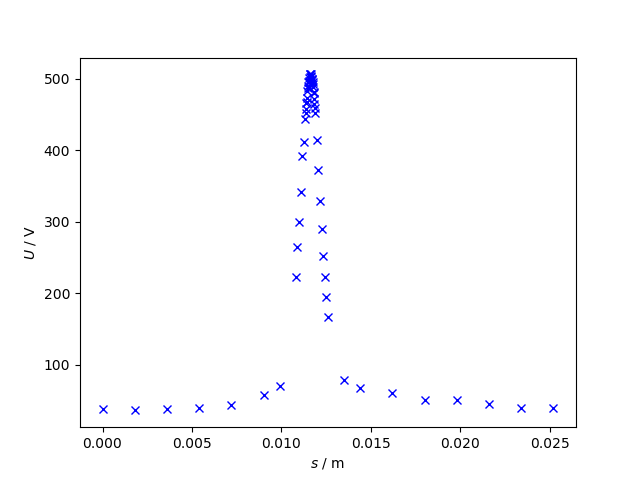
\includegraphics[width=0.8\textwidth]{python/plots/plot_0.png}
\caption{Intensitätsverteilung der Kaliumatome abhängig von der Auslenkung des Detektors ohne Magnetfeld.}
\label{fig:a:0}
\end{figure}
%%%%%%%%%%%%%%%%
\begin{figure}
\centering
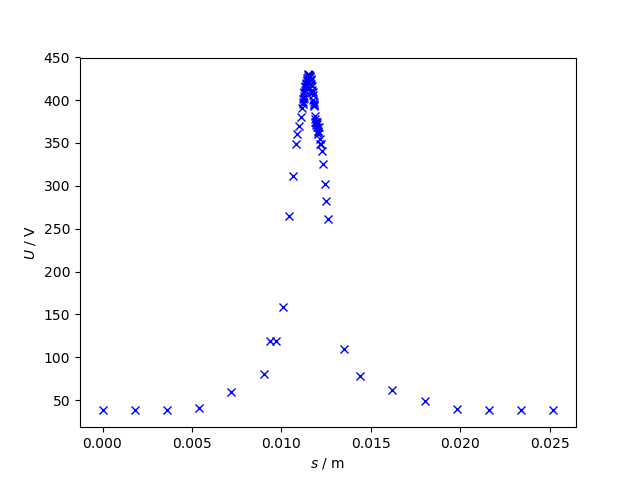
\includegraphics[width=0.8\textwidth]{python/plots/plot_1.png}
\caption{Intensitätsverteilung der Kaliumatome abhängig von der Auslenkung des Detektors mit Magnetfeld $B=\SI{0.11}{\tesla}$.}
\label{fig:a:1}
\end{figure}
%%%%%%%%%%%%%%%
\begin{figure}
\centering
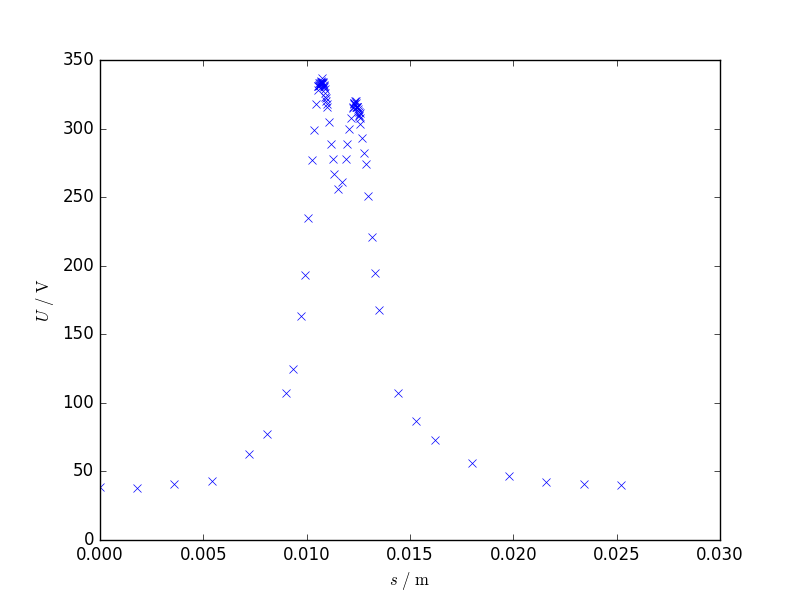
\includegraphics[width=0.8\textwidth]{python/plots/plot_2.png}
\caption{Intensitätsverteilung der Kaliumatome abhängig von der Auslenkung des Detektors mit Magnetfeld $B=\SI{0.23}{\tesla}$.}
\label{fig:a:2}
\end{figure}
%%%%%%%%%%%%%%%%%%%%
\begin{figure}
\centering
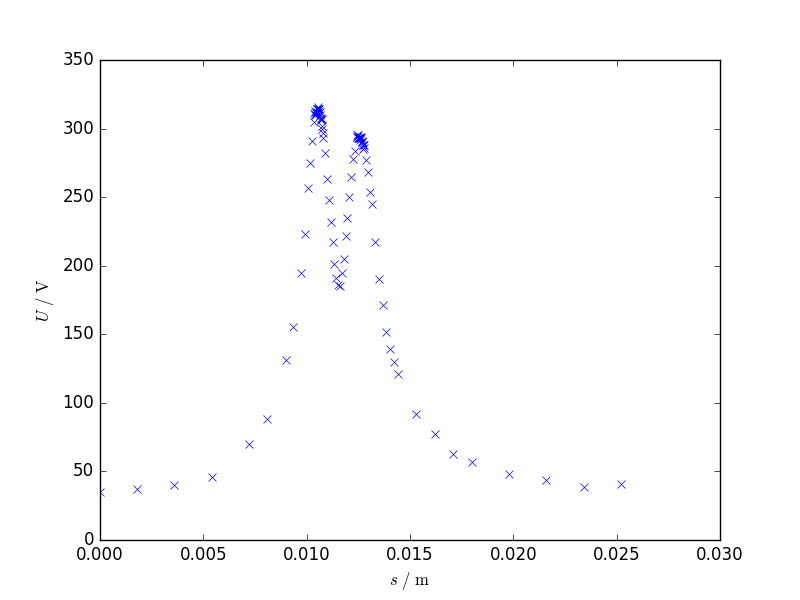
\includegraphics[width=0.8\textwidth]{python/plots/plot_3.png}
\caption{Intensitätsverteilung der Kaliumatome abhängig von der Auslenkung des Detektors mit Magnetfeld $B=\SI{0.30}{\tesla}$.}
\label{fig:a:3}
\end{figure}
%%%%%%%%%%%%%%
\begin{figure}
\centering
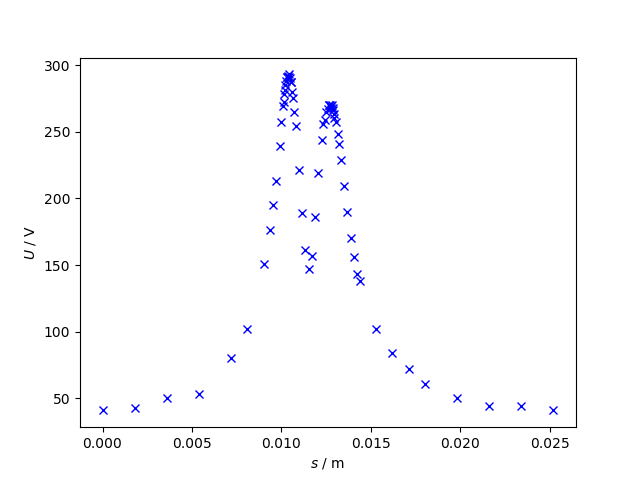
\includegraphics[width=0.8\textwidth]{python/plots/plot_4.png}
\caption{Intensitätsverteilung der Kaliumatome abhängig von der Auslenkung des Detektors mit Magnetfeld $B=\SI{0.38}{\tesla}$.}
\label{fig:a:4}
\end{figure}
%%%%%%%%%%%%%%%%
\begin{figure}
\centering
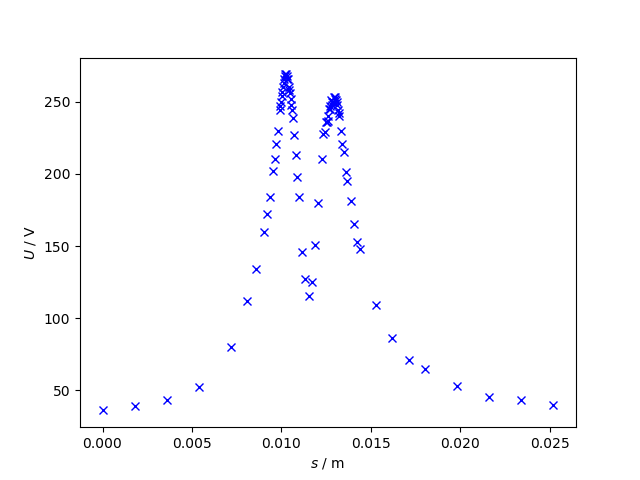
\includegraphics[width=0.8\textwidth]{python/plots/plot_5.png}
\caption{Intensitätsverteilung der Kaliumatome abhängig von der Auslenkung des Detektors mit Magnetfeld $B=\SI{0.45}{\tesla}$.}
\label{fig:a:5}
\end{figure}
%%%%%%%%%%%%%%%%%%%%
\begin{figure}
\centering
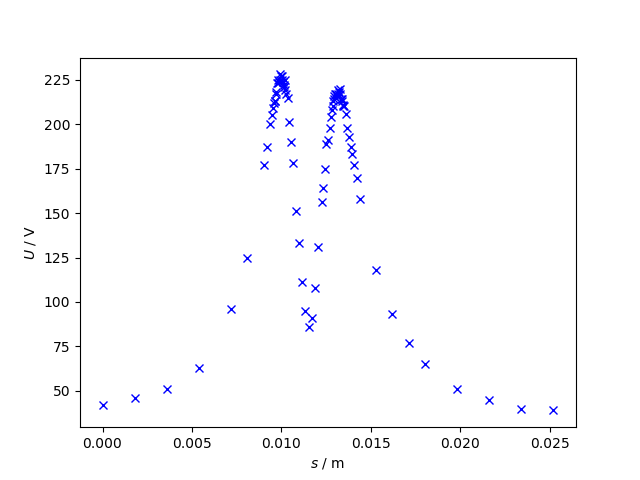
\includegraphics[width=0.8\textwidth]{python/plots/plot_6.png}
\caption{Intensitätsverteilung der Kaliumatome abhängig von der Auslenkung des Detektors mit Magnetfeld $B=\SI{0.59}{\tesla}$.}
\label{fig:a:6}
\end{figure}
%%%%%%%%%%%%%%%%%
\begin{figure}
\centering
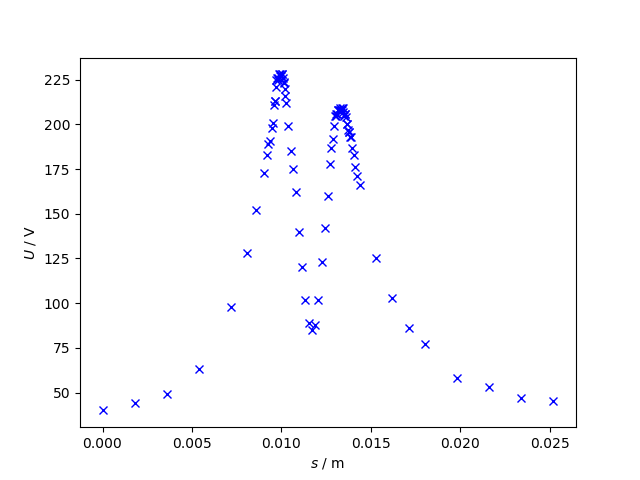
\includegraphics[width=0.8\textwidth]{python/plots/plot_7.png}
\caption{Intensitätsverteilung der Kaliumatome abhängig von der Auslenkung des Detektors mit Magnetfeld $B=\SI{0.65}{\tesla}$.}
\label{fig:a:7}
\end{figure}
%%%%%%%%%%%%%%%%%
Im folgenden werden alle Ausgleichsrechnungen mit der Funktion \textit{curve\_ fit} aus dem Python Paket \textit{scipy} durchgeführt.
Um die Intensitätsmaxima möglichst präzise zu bestimmen, soll eine Ausgleichsrechnung mit der Fitfunktion
\begin{align*}
f(x)=a_1\exp(-b_1(x-c_1)^2) + a_2\exp(-b_2(x-c_2)^2) + d
\end{align*}
durchgeführt werden.
Da die Rechnungen ohne weiteres nicht konvergieren, werden die Positionen der Maxima möglichst präzise mit dem Mauszeiger aus den Diagrammen abgelesen.
Die entsprechenden Werte sind in Tabelle \ref{tab:a:1} aufgeführt.
\begin{table}
\centering
\caption{Gemessene Lagen der Intensitätsmaxima $s_1$ und $s_2$ beim Magnetfeld $B$, sowie die mittleren Abstände $\frac{s_2 - s_1}{2}$ der Maxima von der Nullposition.}
\label{tab:a:1}
\begin{tabular}{c c c c}
\hline
$B$ in T & $s_1$ in mm & $s_2$ in mm & $\frac{s_2 - s_1}{2}$ in mm\\ \hline
0.23 &10.7086  &12.3886  &0.8400  \\
0.30 &10.5543  &12.5965  &1.0211   \\
0.38 &10.3943  &12.7545  &1.1801   \\
0.45 &10.2490 &12.9138  &1.3324   \\
0.59 &10.0221  &13.1821  &1.5800  \\
0.65 &9.9415  &13.2806  &1.66955 \\
\hline
\end{tabular}
\end{table}
Auch mit den abgelesenen Startwerten als Startparameter konvergieren die Rechnungen nicht.
Um die Fitfunktion zu vereinfachen wird $a_1=a_2, b_1=b_2,c_1=c_2$ gesetzt.
Jedoch verbesserte diese Maßnahme das Konvergenzverhalten ebenfalls nicht.
Aus diesem Grund werden im folgenden die abgelesenen Werte verwendet.
In Abbildung \ref{fig:a:8} werden die mittleren Abstände der Intensitätsmaxima von der Nullposition gegen die entsprechenden Magnetfeldgradienten aufgetragen. 
\begin{figure}
\centering
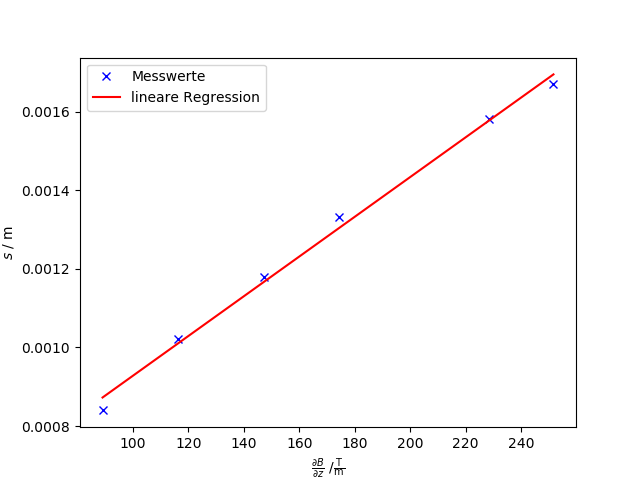
\includegraphics[width=0.8\textwidth]{python/plots/plot_8.png}
\caption{Mittlerer Abstand der Intensitätsmaxima von der Nullposition in Abhängigkeit des Magnetfeldgradienten und die zugehörige lineare Ausgleichsrechnung.}
\label{fig:a:8}
\end{figure}
Dabei wurde die in Abbildung \ref{fig:a:1} dargestellte Messreihe nicht mit einbezogen, da keine Maxima auszumachen waren.
Eine lineare Ausgleichsrechnung liefert für die Steigung der Ausgleichsgerade den Wert $a=\SI{5.05\pm 0.19e-06}{1\per\tesla}$.
Mit Gl. \eqref{eq:t:8} und Gl. \eqref{eq:t:3} folgt für das Bohrsche Magneton der Wert
\begin{align*}
\mu_B = \SI{6.59 \pm 0.25 e-24}{\joule\per\tesla}
\end{align*}
Dabei wurde die Fortpflanzung der Abweichung vom Python Paket \textit{uncertainties} berechnet.